\documentclass[tikz,border=7pt]{standalone}
\usepackage[utf8]{inputenc}
\usepackage[OT4,plmath]{polski}
\usepackage{amssymb}
\begin{document}
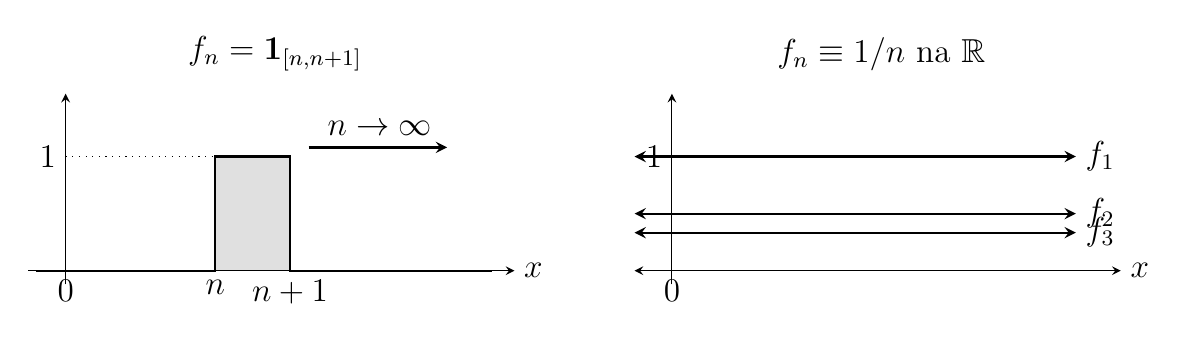
\begin{tikzpicture}[x=0.95cm,y=1.45cm,>=stealth,font=\large]
  \begin{scope}
    \node at (2.8,1.9) {$f_n=\mathbf{1}_{[n,n+1]}$};
    \fill[black!12] (2,0) rectangle (3,1);
    \draw[thick] (-0.4,0) -- (2,0) -- (2,1) -- (3,1) -- (3,0) -- (5.7,0);
    \draw[->] (-0.5,0) -- (6,0) node[right] {$x$};
    \draw[->] (0,-0.12) -- (0,1.55);
    \draw[dotted] (0,1) node[left] {$1$} -- (2,1);
    \node[below] at (0,0) {$0$};
    \node[below] at (2,0) {$n$};
    \node[below] at (3,0) {$n+1$};
    \draw[->,thick] (3.25,1.08) -- (5.1,1.08);
    \node[above] at (4.2,1.1) {$n\to\infty$};
  \end{scope}
  \begin{scope}[xshift=7.7cm]
    \node at (2.8,1.9) {$f_n\equiv1/n$ na $\mathbb R$};
    \draw[<->] (-0.5,0) -- (6,0) node[right] {$x$};
    \draw[->] (0,-0.12) -- (0,1.55);
    \foreach \height/\lab in {1/f_1,0.5/f_2,0.3333/f_3} {
      \draw[<->,thick] (-0.5,\height) -- (5.4,\height);
      \node[right] at (5.4,\height) {$\lab$};
    }
    \node[left] at (0,1) {$1$};
    \node[below] at (0,0) {$0$};
  \end{scope}
\end{tikzpicture}
\end{document}
